\documentclass{article}

\textwidth=6.5in
\textheight=8.5in
\voffset=-54pt
\oddsidemargin=0in
\evensidemargin=0in
\setlength{\parskip}{8pt}
\setlength{\parindent}{0pt}

\usepackage{workbook}

\usepackage[]{handout}

\begin{document}

\begin{center}
  \large\textsc{Problem Set 4 - Implicit Differentiation}

    \pspace{12pt}
  \begin{problemonly}\large Name: \rule{5cm}{0.15mm}\\ \end{problemonly}
\end{center}

  Pages 541 to 548 in Gottlieb contain examples similar to these problems.

  \begin{enumerate}
  \item
\begin{problem}[\vfill]
      Find the equation of the line tangent to the curve
      $x^3+y^3-3x^2 y^2 +1=0$ at the point $(1,1)$.
    \end{problem}

    \begin{solution} 
      The slope of the line is $\frac{dy}{dx}$ at the point $(1, 1)$, and
      we'll use implicit differentiation to find this.
      \begin{align*}
        x^3+y^3-3x^2 y^2 +1&=0\\
        \intertext{Differentiate both sides with respect to $x$ (since we
          want $\frac{dy}{d\bm{x}}$):}
        3 x^ { 2} + \frac{d}{dx}
        \left(\fcolorbox{red}{white}{$\displaystyle
            \fcolorbox{blue}{white}{$\displaystyle  y$}^ {
              3} $}\right)- 3 \frac{d}{dx}
        \left(\fcolorbox{green}{white}{$\displaystyle  x^ { 2} $}\cdot
          \fcolorbox{green}{white}{$\displaystyle  y^ { 2} $}\right) &= 0 \\
        3 x^ { 2} + 3 y^ { 2} \frac{dy}{dx}- 3 \left[x^ { 2} \cdot
          \frac{d}{dx} \left(\fcolorbox{red}{white}{$\displaystyle
              \fcolorbox{blue}{white}{$\displaystyle  y$}^ { 2} $}\right)+
          2 x\cdot y^ { 2} \right] &= 0 \\
        3x^2+3y^2\frac{dy}{dx} - 3x^2\cdot2y\frac{dy}{dx} - 6xy^2 & = 0\\
        \intertext{Now, we can plug in the point $(1, 1)$:}
        3 + 3 \frac{dy}{dx} - 6 \frac{dy}{dx} - 6 &= 0 \\
        -3 \frac{dy}{dx} &= 3 \\
        \frac{dy}{dx} &= -1
      \end{align*}
      So, the slope of the tangent line is $-1$.  Since the line includes
      the point $(1, 1)$, the line has equation $\boxed{y-1 = -1(x-1)}$.
    \end{solution}

  \item
\begin{problem}[\vfill\newpage]
      Find the equation of the line tangent to the curve $(2x^2 + y^2)^2 =
      9x (2x^2 - y^2)$ at the point $(1, 1)$.
    \end{problem}

    \begin{solution} 
      We use the same method as in {{{{\#1}}(a)}}.
      \begin{align*}
        (2x^2 + y^2)^2 &= 9x (2x^2 - y^2) \\
        \intertext{We want to find $\frac{dy}{dx}$ at the point $(1, 1)$,
          so we differentiate both sides with respect to $x$:} %
        \frac{d}{dx} \left(\fcolorbox{red}{white}{$\displaystyle
            \fcolorbox{blue}{white}{$\displaystyle \left(2 x^ { 2} + y^ {
                  2} \right)$}^ { 2} $}\right) &= \frac{d}{dx} \left(
          \fcolorbox{green}{white}{$\displaystyle 9x$}\cdot
          \fcolorbox{green}{white}{$\displaystyle \left(2 x^ { 2} -y^ {
                2} \right)$}\right) \\
        2 (2x^2 + y^2) \left(4x + 2y \frac{dy}{dx} \right) &= 9 (2x^2 -
        y^2) + 9x \left(4x - 2y \frac{dy}{dx} \right) \\
        \intertext{Plug in the point $(1, 1)$:} %
        2 (3) \left( 4 + 2 \frac{dy}{dx} \right) &= 9 (1) + 9 \left(4 -
          2\frac{dy}{dx} \right) \\
        24 + 12 \frac{dy}{dx} &= 45 - 18 \frac{dy}{dx} \\
        30 \frac{dy}{dx} &= 21 \\
        \frac{dy}{dx} &= \frac{21}{30} = \frac{7}{10}
      \end{align*}
      So, the line we're looking for has slope $\frac{7}{10}$ and includes
      the point $(1, 1)$.  Therefore, its equation is $\boxed{y - 1 =
        \dfrac{7}{10} (x - 1)}$.
    \end{solution}

  \item
\begin{problem}[\vfill]
      Find the equation of the line tangent to the curve $y \ln \left(x^2
        y+ e \right) = x$ at the point $(0, 0)$.
    \end{problem}

    \begin{solution} 
      We use the same method as in {{{{\#1}}(a)}}.
      \begin{align*}
        y \ln \left(x^2 y+ e \right) &= x \\
        \intertext{We want to find $\frac{dy}{dx}$ at the point $(0, 0)$,
          so we differentiate both sides with respect to $x$:}
        \frac{d}{dx} \left(\fcolorbox{green}{white}{$\displaystyle
            y$}\cdot \fcolorbox{green}{white}{$\displaystyle \ln\left(x^ {
                2} y+
              e\right)$}\right) &= \frac{d}{dx} (x) \\
        \frac{dy}{dx} \ln \left(x^2 y+ e \right) + y \frac{d}{dx}
        \left(\fcolorbox{red}{white}{$\displaystyle
            \ln\left(\fcolorbox{blue}{white}{$\displaystyle x^ { 2}
                y+ e$}\right)$}\right) &= 1 \\
        \frac{dy}{dx} \ln \left(x^2 y+ e \right) + y \cdot \frac{1}{x^2 y
          + e} \cdot \frac{d}{dx}
        \left(\fcolorbox{green}{white}{$\displaystyle x^ { 2} $}\cdot
          \fcolorbox{green}{white}{$\displaystyle  y$} + e \right) &= 1 \\
        \frac{dy}{dx} \ln \left(x^2 y+ e \right) + y \cdot \frac{1}{x^2 y
          + e} \left( 2x y + x^2 \frac{dy}{dx} \right) &= 1 \\
        \shortintertext{Plug in the point $(0, 0)$:} %
        \frac{dy}{dx} \ln (e) + y \cdot \frac{1}{e} \left( 0 \right) &= 1
        \\
        \frac{dy}{dx} &= 1
      \end{align*}
      So, the line we're looking for has slope $1$ and includes the point
      $(0, 0)$.  Therefore, its equation is $y - 0 = 1 (x - 0)$, or just
      $\boxed{y = x}$.
    \end{solution}

  \item
\begin{problem}
      Match the three curves with their graphs.  (Think about what your previous work tells you.)

        \begin{multicols}{2}
        \begin{enumerate}[topsep=0pt, label=(\arabic*)]
        \item $x^3+y^3-3x^2 y^2 +1=0$

        \item $(2x^2 + y^2)^2 = 9x (2x^2 - y^2)$

        \item $y \ln \left(x^2 y+ e \right) = x$

        \end{enumerate}
        \end{multicols}
      
        \vspace{-6pt}
      Graphs:
      
        \centering
        \begin{tabular}{ccc}
        (A) & (B) & (C) \\
          \begin{minipage}{0.25\textwidth}
          \includegraphics[width=1.5in]{images/implicit-differentiation-matching-1-3}
          \end{minipage}
          &
          \begin{minipage}{0.25\textwidth}
          \includegraphics[width=1.5in]{images/implicit-differentiation-matching-1-1}
          \end{minipage}
          &
          \begin{minipage}{0.25\textwidth}
          \includegraphics[width=1.5in]{images/implicit-differentiation-matching-1-2}
          \end{minipage}

        \end{tabular}
      
    \end{problem}

    \begin{solution} 
      From our work in \#1, we know that the line
      tangent to curve 1 at $(1, 1)$ has negative slope; that matches only
      B.

      From our work in
      \#3, we know
      that the line tangent to curve iii at $(0, 0)$ has slope 1, which
      matches only C.

      Therefore, by process of elimination, we get \fbox{1 - B, 2 - A, 3 - C}. 
    \end{solution}

\pspace{\newpage}

\item
\begin{grading}
10 points, broken down as follows: 3/1/2/2/2
\end{grading}

% Spring 2012 Math Mb
  Gordon has a new puppy, and he is keeping careful track of the puppy's
  height and weight.  So far, the puppy's height $H$ (measured in feet)
  and weight $W$ (measured in pounds) appear to be related by the
  equation $\displaystyle W(H W^2+100)=2000 H$.  The graph of the relationship is shown below.
  
  \begin{center}
  \resizebox{0.3\textwidth}{!}{
    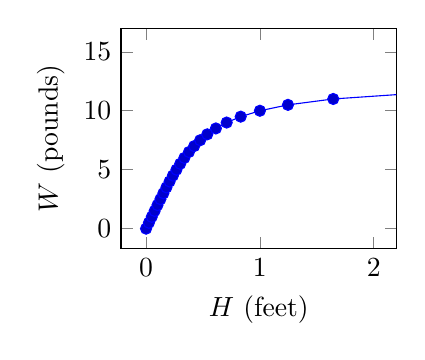
\begin{tikzpicture}
      \begin{axis}[xlabel=$H$ (feet), ylabel=$W$ (pounds), xmax=2.2,
        ymax=17, width=2in] 
        \addplot+[domain=0:12] ({100*x/(2000-x^3)}, x);
      \end{axis}
    \end{tikzpicture}
    }
  \end{center}
  
  \begin{enumerate}
  \item
    \begin{problem}[\vfill]
      When the puppy was 1 foot tall, it weighed 10 pounds.  Find $\frac{dW}{dH}$ at this moment.
    \end{problem}

    \begin{solution} % Jason Bland
      Let's expand the given equation to make it slightly simpler to
      differentiate:
      \begin{align*}
        HW^3 + 100W &= 2000H \\
        \intertext{Now, we'll differentiate both sides with respect to
          $H$ (because we want $\frac{dW}{d\bm{H}}$):} \frac{d}{dH}
        \left(\fcolorbox{green}{white}{$\displaystyle H$}\cdot
          \fcolorbox{green}{white}{$\displaystyle W^ { 3} $} +
          \fcolorbox{purple}{white}{$\displaystyle 100$}\cdot W\right) &= \frac{d}{dH}
        (\fcolorbox{purple}{white}{$\displaystyle 2000$}\cdot H) \\
        W^3 + H \cdot \frac{d}{dH}
        \left(\fcolorbox{red}{white}{$\displaystyle
            \fcolorbox{blue}{white}{$\displaystyle W$}^ { 3} $}\right) +
        100 \frac{dW}{dH}
        &= 2000 \\
        W^3 + H \cdot 3W^2 \frac{dW}{dH} + 100 \frac{dW}{dH} &= 2000 \\
        \intertext{At this point, it's okay to plug in the point $H=1$ and $W=10$:}
        1000 + 300 \frac{dW}{dH} + 100 \frac{dW}{dH} &= 2000 \\
        400 \frac{dW}{dH} &= 1000 \\
        \frac{dW}{dH} &= \boxed{\frac{5}{2}}
      \end{align*}
    \end{solution}

  \item
    \begin{problem}[\stretch{0.2}]
      What are the units of $\frac{dW}{dH}$?
    \end{problem}

    \begin{solution} % Jason Bland
      The units are pounds per foot.
    \end{solution}

    \end{enumerate}


    \begin{framed}
    \textbf{Recall:}
    $\frac{dW}{dH}=\lim\limits_{\Delta H\to 0}\frac{\Delta W}{\Delta H}$.
    So if $\Delta H$ is very small, $\frac{dW}{dH} \approx \frac{\Delta W}{\Delta H}$.
    
    \textbf{Example:} When the puppy was about 0.5 feet tall and weighed about 7.7 pounds, $\diff{W}{H}=8$.
    This tells us that $\frac{\Delta W}{\Delta H} \approx 8$, which we can rearrange as $\Delta W \approx 8\Delta H$. 
    
    In words: for any small change in the puppy's height from 0.5 feet, the corresponding small change in the puppy's weight from 7.7 pounds was about eight times as large.
    \end{framed}


    \begin{enumerate}[resume]

  \item
    \begin{problem}[\stretch{0.5}]
      Use the value you found for $\frac{dW}{dH}$ to approximate the puppy's weight when it was 1.1 feet tall.
    \end{problem}

    \begin{solution}
      In part (a), we found that when $H=1$ and $W=10$, $\frac{dW}{dH}=2.5$.
      This means that $\Delta W \approx 2.5 \Delta H$. Since $\Delta H = 0.1$,
      $\Delta W \approx 2.5 \cdot 0.1 = 0.25$. This means that a reasonable
      estimate for the puppy's weight when it's 1.1 feet tall is $\boxed{10.25 \text{ pounds}}$.
    \end{solution}

  % \item
  %   \begin{problem}[\stretch{0.5}]
  %     Find an equation for the line tangent to the graph at the point $(1, 10)$.
  %     Use point-slope form.
  %   \end{problem}
    

  %   \begin{solution} % Jason Bland
  %     This is the line through $(1, 10)$ having a slope of
  %     $\frac{5}{2}$. Its equation is $\boxed{W - 10 = \frac{5}{2}(H -
  %       1)}$.
  %   \end{solution}

  % \item
  %   \begin{problem}[\nstretch{0.5}]
  %     Using the equation of the tangent line, approximate the puppy's weight when it was 1.1 feet tall.\\
  %     \emph{Note: Your answers to (c) and (e) should agree.}
  %   \end{problem}


  %   \begin{solution} % Jason Bland
  %     The idea of linear approximation is simply that the tangent line
  %     we found is a very good approximation for the actual curve near
  %     the point $(1, 10)$.  That is, for $H$ near 1,
  %     \[ 
  %     W \approx 10 + \frac{5}{2}(H - 1).\] In particular, when $H =
  %     1.1$, $W \approx 10 + \frac{5}{2}(0.1) = \boxed{10.25}$ pounds.
  %   \end{solution}

  \end{enumerate}

\pspace{\newpage}

\item
\begin{grading}
3 points.
\end{grading}

 \textbf{Reflect back.}

  \begin{problem}
    Akiko, Chomei, and Emi are trying to find the slope of the line
    tangent to the curve $3x^2 + 2xy + y^2 = 3$ at the point $(1, 0)$.
    They are trying to decide on a strategy for solving this problem.
    \begin{itemize}
    \item Akiko thinks they should plug in $x = 1$, $y = 0$ right away,
      then differentiate both sides of the equation with respect to $x$ and solve for $\frac{dy}{dx}$.
    \item Chomei thinks they should first differentiate both sides of the
      equation with respect to $x$, then plug in $x = 1$, $y = 0$ and solve
      for $\frac{dy}{dx}$.
    \item Emi thinks they should first differentiate both sides of the
      equation with respect to $x$, then solve for $\frac{dy}{dx}$ (in terms
      of $x$ and $y$), and then plug in $x=1$, $y=0$ to find a value.
    \end{itemize}
  \end{problem}
    
    \begin{enumerate}
        \item
        \begin{problem}
            One of these strategies does not work. Which one?
        \end{problem}
        \pspace{\vfill}

        \begin{solution}
    Akiko's method does not work. If we start by plugging $x = 1$, $y =
    0$ into $3x^2 + 2xy + y^2 = 3$, we just get the equation $3 = 3$.
    Differentiating this doesn't tell us anything about $\frac{dy}{dx}$.
    The problem is that $\frac{dy}{dx}$ is talking about a rate of change:
    how $y$ changes with respect to $x$. Plugging $x = 1, y = 0$ in means that the equation only represents the relationship between $x$ and $y$ at that one specific point, and we can't use it to determine how $x$ and $y$ are changing.
        \end{solution}

        \item 
        \begin{problem}
           Of the strategies that work, whose requires less algebra?
        \end{problem}
        \pspace{\vfill}

        \begin{solution}
            Chomei's strategy is correct and computationally simpler than Emi's. If we plug in values for $x$ and $y$ immediately after differentiating, then we the algebra of solving for $\frac{dy}{dx}$ is not as complicated.
        \end{solution}

        \item
        \begin{problem}
            Of the strategies that work, whose would be efficient for finding the slope at many different points?
        \end{problem}
        \pspace{\vfill}

        \begin{solution}
            Emi's strategy is correct, and although it is algebraically more involved than Chomei's, it leads to a formula for $\frac{dy}{dx}$ that we can reuse with many different points.
        \end{solution}
    \end{enumerate}
    

  \begin{solution}


    Chomei and Emi's methods both work, but Chomei's is computationally
    simpler.
  \end{solution}


\item We will learn a new method of differentiation next class that will help us find the derivative of $f(x)= x^x$. Let's first investigate this function in this problem. The graph of $y=f(x)$ is shown below.

\begin{minipage}[t]{2in}\vspace{0pt}
      \begin{tikzpicture}
          \begin{axis}[xlabel=$x$, ylabel=$y$, height=4in, width=2in,
          xtick={1,2,3}, ytick={1,4,27}, clip=false, ymax=30]
              \addplot[domain=0:3.05,->] {x^x};
              \addplot[closed] coordinates {(0,1) (1,1) (2,4) (3,27)};
              \node[above] at (1,1) {$(1,1)$};
              \node[right] at (2,4) {$(2,4)$};
              \node[left] at (3,27) {$(3,27)$};
          \end{axis}
      \end{tikzpicture}
\end{minipage}
\begin{minipage}[t]{4in}
\begin{enumerate}
    \item
    \begin{problem}
        Use the graph to determine the domain of the function.
    \end{problem}
    \pspace{36pt}

    \begin{solution}
        The domain is $[0,\infty)$.
    \end{solution}

    \item
    \begin{problem}
        Find an upper bound and a lower bound for the value of $f'(2)$ by calculating slopes.
    \end{problem}
    \pspace{2in}
    
    \begin{solution}
        $f'(2)$ is the slope of the line tangent to the graph at $(2,4)$. From the graph, we can tell that this slope is greater than the slope of the secant line between $(1,1)$ and $(2,4)$, which is $3$.

        We can also tell from the graph that $f'(2)$ is less than the slope of the secant line between $(2,4)$ and $(3,27)$, which is $23$.

        Therefore we know that $3 < f'(2) < 23$.
    \end{solution}
    
\end{enumerate}
\end{minipage}

\pspace{\newpage}

  \begin{enumerate}[resume]
  \pspace{18pt}
  \item
\begin{problem}
      Fill in the limit definition of $f'(2)$: $f'(2) = \displaystyle
      \lim_{h \to 0} \fitb[\vphantom{\frac{0}{0}}]{3in}{\frac{f(2 + h) - f(2)}{h}}$.
    \end{problem}
\end{enumerate}

In parts (e)-(g), use a calculator to give decimal approximations.

\begin{enumerate}[resume]
  \item
\begin{problem}[\vfill]
      Approximate $f'(2)$.  (Hint: $f'(2)$ is the value of a specific limit as $h \to 0$. To \emph{approximate} $f'(2)$, you can plug
      in a value of $h$ which is very close to $0$.)
    \end{problem}

    \begin{solution} % Jason Bland
      We could approximate by plugging in values of $h$ such as $0.001$
      and $-0.001$: 
      \begin{align*}
        \frac{f(2 + 0.001) - f(2)}{0.001} &= \frac{(2 + 0.001)^{2 +
            0.001} - 4}{0.001} % = 1000 \Big( 2.001^{2.001} - 4 \Big)
        \approx 6.779 \\
        \frac{f(2 - 0.001) - f(2)}{-0.001} &= \frac{(2 - 0.001)^{2 -
            0.001} - 4}{-0.001} % = 1000 \Big( 4 - 1.999^{1.999} \Big)
        \approx 6.766 
      \end{align*}
      This suggests $f'(2)$ is about $6.77$.
    \end{solution}

  \item
    \begin{problem}[\vfill]
      If we naively tried to treat $f(x)=x^x$ like a power function, we
      might think that $f'(x) = x\cdot x^{x-1}$.  Based on what you know about $f'(2)$, explain why $f'(x)\neq x\cdot x^{x-1}$.
    \end{problem}

    \begin{solution} % Jason Bland
      This would suggest $f'(2) = 2 \cdot 2^{2 - 1} = 4$ which is not
      at all close to $6.77$.
    \end{solution}

  \item
    \begin{problem}[\vfill]
      If we naively tried to treat $f(x)$ like an exponential function, we might think that $f'(x) = x^{x} \cdot \ln(x)$.  Based on what you know about $f'(2)$, explain why $f'(x)\neq x^x \cdot
      \ln(x)$.
    \end{problem}

    \begin{solution} % Jason Bland
      This would suggest $f'(2) = 4 \ln 2 \approx 2.77$, which is also
      not close to $6.77$.
    \end{solution}

  \end{enumerate}

\end{enumerate}



\psreflection{
    The optional reading for next class is pp. 537-538 in Gottlieb.
}

\end{document}